% TARI29_Assignment_report_template.tex
% This is a template for the assignment reports
% TARI29 Artificial Intelligence, 7.5 credits, Winter 2024
% Original version by:  Vladimir Tarasov, 2024
% Revised by:		   Alexandros Tzanetos, 2024 

% Use a modern class instead of an old article class
\documentclass{scrartcl}

\KOMAoptions{
	parskip=half,  % full, off
	fontsize=12pt, % base font size (10pt default)
	% headings=big,% small/normal/big headings (normal is default), 
	% paper=a5,	% paper format (a4 default) 
	pagesize=auto  % Use paper format for PDF too
}

% ---------------------- Report details --------------------- %
%\newcommand{\docauthor}{Name1, Name2, Name3}
\newcommand{\courseyear}{2024}
\newcommand{\coursename}{TARI29 Artificial Intelligence}
\newcommand{\coursecredits}{7.5 credits}
\newcommand{\fullcoursename}{\coursename, \coursecredits}
\newcommand{\termname}{Winter \courseyear}
\newcommand{\groupnumber}{24}
\newcommand{\reportname}{Group \groupnumber\ Assignment Report}
\newcommand{\assignmentname}{Evolutionary Computation Assignment}
% ------------------ End of report details ------------------ %



% ---------- Setting up properties of the PDF file ---------- %
\usepackage{hyperref}
\hypersetup{
	colorlinks=true,
	allcolors=blue,
	pdftitle={\reportname},
	pdfauthor={Oskar Sundberg, Linus Savinainen, Samuel Wallander Leyonberg, Gustav Pråmell, Joel Scarinius Stävmo},
	pdfsubject={\coursename, \termname}
	% pdfpagemode=FullScreen,
	% pdfpagemode= UseOutlines % the default if present
}
% ------------ End of properties of the PDF file ------------ %



% ----------- Setting up the headers and footers ------------ %
\usepackage{scrlayer-scrpage}
\pagestyle{scrheadings}
\KOMAoptions{% 
	headsepline,% line below the header
	plainheadsepline,% also on scrplain
}
\clearpairofpagestyles % Erase all current configurations
% inner part of the header [titel_page]{other_pages}
\ihead[\coursename, \courseyear]{\coursename, \courseyear}
% outer part of the header [titel_page]{other_pages}
\ohead{\assignmentname}
% center part of the footer [titel_page]{other_pages}
\cfoot[\textup{Page \pagemark\ of \ztotpages}]{\textup{Page \pagemark\ of \ztotpages}}
% ------------- End of the headers and footers -------------- %



% ---------------- Setting up the title page ---------------- %
\title{\reportname}
\subtitle{An Evolutionary approach to elevator time optimization}
%\author{\docauthor}
\author{Oskar Sundberg \and Linus Savinainen \and Samuel Wallander Leyonberg \and Gustav Pråmell \and Joel Scarinius Stävmo}
\date{\today}
% ------------------ End of the title page ------------------ %



% --------------- Packages and custom commands -------------- %
% Specify the input encoding of the source file as UTF8 
\usepackage[utf8]{inputenc}
% The T1 font encoding is an 8-bit encoding and fully supports words containing accented characters
\usepackage[T1]{fontenc}
% Load Latin modern fonts in outline format
\usepackage{lmodern}
% Load better typewriter font
\usepackage{inconsolata}
% For better hyphenation patterns
\usepackage[english]{babel}
% For improved micro-typography
\usepackage{microtype}
% Switch off extra space after a sentence
\frenchspacing
% To be able to include pictures
\usepackage{graphicx}
\usepackage{zref-totpages} % To get the total number of pages
\usepackage{mathtools,amsmath} % for advanced math formulas
% To highlight source code
\usepackage{minted}
% Default options for all minted environments
\setminted{
			style=default, % for minted envronment
			autogobble, % automatically remove all common leading whitespace
			xleftmargin=10pt, % indentation to add (on the left) before the listing
			numbersep=6pt, % gap between numbers and start of line
			linenos, % enables line numbers
			mathescape % enables the usual math mode inside comments
}
\setmintedinline[c]{style=default} % for minted inlines
% Flexible handling of verbatim text
\usepackage{fancyvrb}
% For well-spaced lines and guidelines in tables
\usepackage{booktabs}
% To typeset algorithms or pseudocode in LaTeX 
\usepackage{algorithm}
\usepackage{algpseudocode}
% For plots and graphs
\usepackage{pgfplots}
\pgfplotsset{width=10cm,compat=1.9}
% To be able to place figures side by side
\usepackage{subcaption}
% This package is used to reference the last page of the document.
\usepackage{lastpage}
% ----------- End of packages and custom commands ----------- %

\begin{document}

\maketitle

\newpage

\tableofcontents

\newpage

\section{Introduction}
\label{sec:intro}
\textcolor{red}{The recommended software for typesetting assignment reports is \LaTeX. It will allow you to prepare high-quality documents, especially in the area of Computer Science. This document can serve as a template for reports. Each section begins with brief instructions in red text. All the instructions in red, as well as the dummy text, should be removed in the final version to submit. The \LaTeX\ source of this file includes examples of using the most needed commands and environments. You can find plenty of other examples with explanations in many web forums and discussion groups on the Internet. The easiest way to edit your report is to use \url{https://www.overleaf.com/}. Overleaf does not require any setup on your computer, and it is free to create an account.}

\textcolor{red}{The book \textit{Writing for Computer Science} \cite{zobel2014writing} is a useful assistance on how to write properly and present your work when it comes to Computer Science topics. It is a strong recommendation to follow its guidelines and limit the usage of AI tools to generate text. Keep in mind that the examiner is an expert in Evolutionary Computation and therefore, any false information generated by an AI tool is easily notable. Such case may lead to failing the assignment.}

\textcolor{red}{The introduction should briefly introduce the assignment and its purpose.}

This report addresses an investigation for optimizing an elevators route to improve the efficiency of picking up and delivering passengers to their desired floors in the least amount average waiting time.
In large buildings with a lot of floors, efficient elevators are crucial for managing traffic and must serve every one in a reasonable time.
Poorly designed elevator systems will lead to long waiting time, unnecessary stops and unsatisfied users.
Elevator technology have made progress during the years, but many elevators still struggle with finding an efficient way
to serve passengers.

The hypotheses that evolutionary algorithms will be able to find near-optimal or optimal routes for elevators
aiming to maximize the number of passengers served while minimizing travel distance and/or travel time is
the core focus in the report. Different strategies and hyperparameter are experimented with to enable
demonstration of how evolutionary algorithms can be used in such a problem. 

This paper will focus on a statically defined problem, i.e., there will not be more passengers coming to the elevator as time goes on, unlike a normal elevator. 


\newpage

\section{Optimize elevator routing}
\label{sec:problem_description}
% Author: Joel Scarinius Stävmo, Oskar Sundberg, Linus Savinainen, Samuel Wallander Leyonberg  and Gustav Pråmell
% Update: October 1, 2024
% Version: 1.0.0
% License: Apache 2.0

\subsection{Mathematical formulation}
% Author: Joel Scarinius Stävmo, Oskar Sundberg, Linus Savinainen, Samuel Wallander Leyonberg  and Gustav Pråmell
% Update: October 1, 2024
% Version: 1.0.0
% License: Apache 2.0

\textbf{Diffing a lower bound}:

Dn = distance needed, Dt = distance travled, N is the number on persons in the building and F = number off floors.(using zero index)

\textbf{Assumption I}: The distance between any floor J and J+1 or J and J-1 is one and the time required is one.

\textbf{Assumption II}: Following I, a person need to go from floor J to floor J+3, the Dn is equal to |J-(J+3)|.

\textbf{Assumption III}: The elevator has the capacity of N.

\textbf{Assumption IV}: For N persons that starts on the same floor and needs to go to the same floor, the lowest time spent waiting is equal to Dn*N.

\textbf{Proof}:
To prove Assumption IV:
Trivial case: A building with F = X and N = 0, there is no need to move the elevator. Resulting in 0*N=0, the Dn*0 = time = 0.

\textbf{Simple case}: A building with F = 2 and N = 1, where the person needs to move for floor zero to floor one. It is trivial to see that the best solution is for the elevator to take one person from floor 0 to floor one. Resulting in Dn = time = 1 = Dt*1.

\textbf{A more general case}:
A building with 2 floor and N person that need to move from floor zero to floor one. The optimal solution is, N*Dn = N*Dt = Time = N.

This is the lower bound of our problem, by proving IV, it can be shown that the lower bound is Dn*N.

\textbf{The upper bound}}:
To prove the upper bound the following solution can be imagined.

A building with F = 3, N = 1, the person is on floor 0 and like to go to floor 2. The elevator picks up the person but never goes to floor 2, instead the elevator moves between floor zero and floor one for ever. Resulting is  1 * \infty  =   \infty.

\newpage

\cite{anily1992swapping}, "Each vertex of a graph initially may contain an object of a known type. A final state, specifying the type of object desired at each vertex, is also given. A single vehicle of unit capacity is available for shipping objects among the vertices. The swapping problem is to compute a shortest route such that a vehicle can accomplish the rearrangement of the objects while following this route."
\section*{Mapping the elevator problem to the swapping problem.}
\begin{itemize}
	\item Vertices are represented as floors in the elevator.
	\item The object is defined as a person.
	\item Initial state consists of N persons waiting at the floors.
	\item The final state is reached when all persons are at their destination floor.
	\item The elevator is a vehicle with a max capacity that moves the persons between floors, i.e. a single vehicle shipping objects among the vertices.
	\item The elevator problem is aiming to reduce the waiting time of the persons in the elevator and thereby reduce the distance traveled.
\end{itemize}



\newpage
\subsection{Similar published academic work}
2.2 
A Genetic Algorithm Based Elevator Dispatching Method For Waiting Time Optimization \cite{tartan2016genetic} explains how they solve a similar problem but with multiple elevators (what they call cars) instead of our one elevator per building. This paper has been our starting point in terms of algorithms and our approaches by following their flow chart provided in the paper.  
 
The paper describes a \%21 improvement with their methods compared to Ghareib paper \cite{gharieb2005optimal} on the same problem. As this problem is not interlay equal to ours, comparison with this would not give a representee outcome. However, by following the approach in the paper we can run our own simulations for our problem space and compare the results to results given with (theoretically) more suited genetic operations.

INVESTIGATION OF OPTIMIZATION TECHNIQUES ON THE ELEVATOR DISPATCHING PROBLEM \cite{ahmed2022investigation} investigates for different approaches in terms of algorithm to the problem at hand.  One of there algorithm to solve the elevator dispatching problem is a genetic algorithm where they use Davis-order crossover, swap mutation and calculate average time for occupants  witch is used as fitness function. There building (problem space) and predefined settings where as following: 
  
The results from their test show that GA where the best performing algorithm for this problem with the definitions above. 
 
This paper presents results that we later compare to ours with our first implementation as given of the flow chart\cite{tartan2016genetic} as well as later implementation with updated genetic operations. Given their result for testing different algorithms on the problem, a genetic algorithm approach seems to contribute with the best result to the elevator dispatching problem.
Crossover and Mutation Operators of Genetic Algorithms \cite{ahmed2022investigation} lists and shortly describes different types of crossover and mutation operations. They describe Wright's heuristic crossover and categorized it as one of the crossover functions how’s offspring are “in the exploration region near the parents” \cite{ahmed2022investigation}. This reduce premature offspring by overcoming local maximum. On further investigation into different implementations of heuristic crossover, the concept seamed as a good crossover function for our problem due to its simplicity and ability to be largely modified to suit our problem and fitness function.




\subsection{Why this evolutionary approach}
Approach
Our starting point was highly inspired from the flowchart above[1]. Our idea was to implement this as a first approach to have a working code base and to be able to easily switch between genetic operations for experimental reasons. From the papers mentioned in 2.2 Similar papers, a conclusion was drawn that a heuristic crossover would suit our problem for it could be implemented to swap larger sections of genes from different parents. This would be important due to the fact that it is certain sequences of genes that will contribute towards a better result rather than single genes. Our fitness function was at first implementation only focused on giving points for delivering a passenger to its desired floor. This was to make sure that every passenger would arrive. However, we later changed this to have our fitness function take the time spent for the passengers instead together with a penalty time for not delivering a passenger to its destination. Our mutation function plays a fundamental role and is quite aggressive. It swaps genes and can increase or decrease the size of the chromosome. We choose this for avoiding local maximums found by our crossover function. As our implementation of a heuristic crossover function takes larger sequences out of one parent, our thought was that this would not give an explorational function, thus bringing the need for a more aggressive mutation function to compensate for this.




\newpage

\section{Algorithm}
\label{sec:algorithm}
% Author: Joel Scarinius Stävmo, Oskar Sundberg, Linus Savinainen, Samuel Wallander Leyonberg  and Gustav Pråmell
% Update: October 1, 2024
% Version: 1.0.0
% License: Apache 2.0

\subsection{Evolutionary approach}
% Clearly describe the algorithm you developed. You
% should clearly explain the evolutionary operators you used and what modifications
% you did to match the problem. It is extremely important to present also a pseudocode
% of your algorithm.

    The genetic algorithm implemented in this study is based on the framework presented in a relatively recent paper \cite{tartan2016flow}, which explored a similar problem. The details of the implemented genetic algorithm can be found in \ref{alg:pseudocode_ga}. A key difference in this paper is the absence of a termination criterion; instead, the algorithm is set to execute for a specified number of generations.

    \begin{algorithm}
        \caption{Genetic Algorithm}\label{alg:pseudocode_ga}
        \begin{algorithmic}
        \Require $g \geq 0$
        \State Initialize a new population
        \State $g \gets 0$
        \While{\text{g} $ < $ \text{generation limit}}
            \For{\text{all genomes in population}}
                \State Execute the genome on its people
            \EndFor
            \State Calculate the fitness of the population
            \State Sort the population
            \If{\text{want elitism}} \Comment{Start prepairing the next generation}
                \State Bring some of the best genomes to the new population
            \EndIf
            \While{\text{the size of the new population} $ < $ \text{population size}}
                \State Select two parents from the old population
                \If{the crossover chance is fulfilled}
                    \State Breed two children using a crossover operator
                \Else
                    \State Select the two parents as the two new children
                \EndIf
                \For{\text{each child}}
                    \If{the mutation chance is fulfilled}
                        \State Apply a mutation operator
                    \EndIf
                \EndFor
                \State Append the two children to the next population
            \EndWhile
        \EndWhile
        \end{algorithmic}
    \end{algorithm}

\subsubsection{Selection}
% Explain selection algorithm(s)

    The chosen selection algorithm is rank-based selection, and the basic idea behind it is to choose two parents based on their ranks rather than their raw fitness values. For example, if the population consists of six genomes, the best genome is given rank six, the second best rank five and so on. The worst genome is given rank one. Each genome is then given a probability $ P_i $ to be chosen based on their respective ranks, expressed as:

    $$ P_i = \frac{\text{rank}_i}{\sum \text{ranks}} $$

    That is, the best genome would have a probability of $ P_6 = \frac{6}{21} $ to be chosen, the second best $ P_5 = \frac{5}{21} $, and the worst genome $ P_1 = \frac{1}{21} $.

\subsubsection{Crossover}
% Explain crossover algorithm(s)

	The first basic crossover operator is one that simply swaps the last halves of the parents, while respecting the possibility that the length of the two parents may be of different length. For example, if the two parents are $$ [1, 2, 3, 4], [5, 6, 7, 8, 9, 10] $$ the resulting children would be $$ [1, 2, 8, 9, 10], [5, 6, 7, 1, 2] $$

    % !!! TODO: Samuel text here !!!
    Samuel's text here pls

\subsubsection{Mutation}
% Explain mutation algorithm(s)

	Three basic mutation operators were implemented. Firstly, a swap mutation where two randomly chosen floors are swapped. Secondly, an operator which increases the length of the genome by appending a random floor at the end. Lastly, an operator that decreases the length by removing a randomly chosen index of the genome. With these three operators, an additional two operators were constructed by combining the effects of swap and either length operator.

% \subsubsection{Replacement} % Elitism
% We never used elitism in the experiments?

\subsection{Solution representation}
% Clearly describe the solution representation you used.
% You can use figures to improve the comprehensibility of this part.

    Given the nature of this problem, there is not a typical direct solution representation approach as seen in e.g. the knapsack problem, where the solution representation is also directly what is being manipulated in the genetic algorithm. In this paper's elevator problem, the genome is a sequence of floors in which the elevator travels to with the goal to deliver as many people. This situation forced a 'two-way' representation, where the fitness of a genome is reflected upon a list of people. Thus it was decided to encapsulate the list of floors and the list of people under a single class 'Genome' as the solution representation.

\subsection{Fitness function}
% It is also very important to mention the fitness function you
% used. In many cases, the objective function of the problem is not the same as
% the fitness function used in an evolutionary algorithm

    After some basic trial and error, and more importantly, a healthy discussion with the assignment teacher, it was decided to exclusively punish unwanted behaviour of the genome instead of giving rewards or mixing rewards with punishments. As the ultimate goal of the algorithm is to deliver all passangers in a short average time, a punishment-only approach acts like a 'catch-all' sink. Instead of trying to find and giving rewards for all of the different kinds of positive behaviours, it is instead easier to punish any and all negative behaviours. For example, if a passanger wants to travel from floor five to one, that requires an absolute minimum of four floors worth of travel. The implemented fitness function would in that case punish based on the difference in distance needed and the distance that was actually traveled by the passanger. Another simple example would be to punish the genome for everyone that did not arrive at their destinations, rather than rewarding for those that did arrive.



% Text from Joel :))

% Each genome has a score that is increased with one time unit for each person that has not arrived to their desired floor for each floor traveled by the elevator. The fitness function helps to keep track of each genome's score and gives time penalties for each person that has not arrived to their desired floor. The penalties increases the score with 100 which is a severe penalty to promote the algorithm to serve as many people as possible.

% When we used our first and most primitive crossover that simply swaps the last halves of two parents genomes the best fitness value we achieved in five runs was 205 but in this graph we show the worst case score of 10227 when it missed serving one person and received a big penalty. We then decided to try a new crossover that creates the first offspring with gene-by-gene selection and which parent to select a gene from is determined by a weighted random choice based on their fitness scores. The second offspring is created by reversing the first offspring.
% The first crossover reached the best value within fewer generations and seems to preform better in this instance. To be completely sure that we couldn't get improved results by changing to a different crossover without changing anything else we decided to try a much more advance crossover that had a great impact on. 

% The third crossover uses segment-based selection instead of selecting genes individually, this method selects contiguous segments of genes from each parent. The offsets determine how many genes to take from each parent based on their fitness scores. This one always performs well and never get stuck in local minima for long. The best score we achieved with this crossover was 172.


\newpage

\section{Experimental part}
\label{sec:experimentation}
% Author: Joel Scarinius Stävmo, Oskar Sundberg, Linus Savinainen, Samuel Wallander Leyonberg and Gustav Pråmell
% Update: October 1, 2024
% Version: 1.0.0
% License: Apache 2.0

This section describes the setup of experiments:

Each experiment consists of two JSON files; one representing the building which specifies where all people are located, and another containing the population with a set of initial genomes.
These experiments are saved to files rather than being generated randomly each time to ensure the ability to run the same experiment multiple times for consistency.

One specific building which already had result data available was used to compare this algorithm's results against previously known results.

To thoroughly evaluate the algorithm it was decided to test it on buildings of different sizes (small, medium, large) and with corresponding population sizes.
Given the number of experiments required to be run, buildings with 10, 50, and 100 floors containing populations of 10, 50, and 100 people respectively was selected. Additionally, the specific building mentioned earlier which has 21 floors and 10 people was included.

Buildings were generated with constraints ensuring that each floor could hold between 0 and half of the maximum population.
While it was theoretically possible for all people to be on just two floors in practice the distribution was more balanced. For example, in the small 10-floor building with 10 people the distribution was as follows:

\begin{center}
	\begin{tabular}{c c c}
		\textbf{From} &       & \textbf{To} \\
		\hline
		0             & $\to$ & 6           \\
		0             & $\to$ & 8           \\
		3             & $\to$ & 5           \\
		4             & $\to$ & 7           \\
		5             & $\to$ & 7           \\
		6             & $\to$ & 2           \\
		7             & $\to$ & 0           \\
		8             & $\to$ & 4           \\
		9             & $\to$ & 0           \\
		9             & $\to$ & 2           \\
	\end{tabular}
\end{center}

After generating and validating all buildings and populations, the experiments were run. Each experiment was conducted on a computer with an AMD Ryzen 7 7800X3D and took roughly ten seconds to a minute. In total 150 experiments were run.
\newpage
All experiment used the following settings 

\begin{itemize}
    \item \textbf{Generations:} 1000
    \item \textbf{Population size:} 100
    \item \textbf{Crossover methods:} Heuristic single, Heuristic sequence, Swap crossover
    \item \textbf{Mutation methods:} Increase, Decrease, Swap, Swap and Increase, Swap and Decrease
    \item \textbf{Elitism rate:} 0.1
    \item \textbf{Crossover rate:} 1.0
    \item \textbf{Mutation rate:} 0.1, 0.6
	\item \textbf{Elevator capacity:} 8
\end{itemize}


Due to time constraints the only parameter that was adjusted during the experiments was the mutation rate to limit the number of results to analyze.
To ensure the reliability of results each combination of building and population was tested five times allowing to identify potential anomalies. Experiments were conducted with two mutation rates, 10\% and 60\%, to observe differences in algorithm performance.
The thought process behind the very high mutation rate was to semi-simulate the effects of a longer generation limit without significantly increasing runtime.

The experimental procedure is outlined as follows:

\begin{itemize}
	\item Generate the building and population, or load a pre-existing experiment.
	\item Run the experiment generating a CSV file with results and a PNG with a graph.
	\item Re-run the same experiment with different parameters.
	\item Analyze the results to evaluate the algorithm's performance.
\end{itemize}


\newpage

\section{Results and Analysis}
\label{sec:results-analysis}
% Author: Joel Scarinius Stävmo, Oskar Sundberg, Linus Savinainen, Samuel Wallander Leyonberg  and Gustav Pråmell
% Update: October 1, 2024
% Version: 1.0.0
% License: Apache 2.0

The following results are presented using graphs to illustrate key insights from the experiments conducted. The blue line and text represents the simplest crossover method, that swaps the last halves of two parents to create two children described in \ref{par:swap last halves}. The red represents the second crossover method, which selects genes from each parent based on their fitness scores, detailed in \ref{par:swap single genes}. The orange represents the third crossover method, that selects contiguous gene segments from each parent based on their fitness scores, outlined in \ref{par:swap sequnce of genes}.

\subsection{Building Small}
Figure \ref{fig:Building Small results} presents the results for 100 people in the building, as well as the worst performance from five runs for each crossover on the smallest building configuration with 10 people. Figure \ref{fig:Building Small worst} displays the worst case in these runs where the blue crossover failed to serve one person and incurred a large penalty. To highlight that with more people in a building, the orange crossover kept getting good results with great consistency Figure \ref{fig:Building Small 100 people} was used. The blue acted comparably, but it wasn't as consistent. The red one was highly unreliable, occasionally achieved positive results on the other hand, it frequently got stuck in local minimums for extended durations. Besides that it took more generations for all crossovers to reach an acceptable solution because of the increased number of people. The orange and blue crossover often reached a good solution quicker than the red one, which also tends to get worse the more people it has to serve.

\begin{figure}[ht]
	\centering
	\begin{subfigure}[b]{0.49\linewidth}
		\centering
		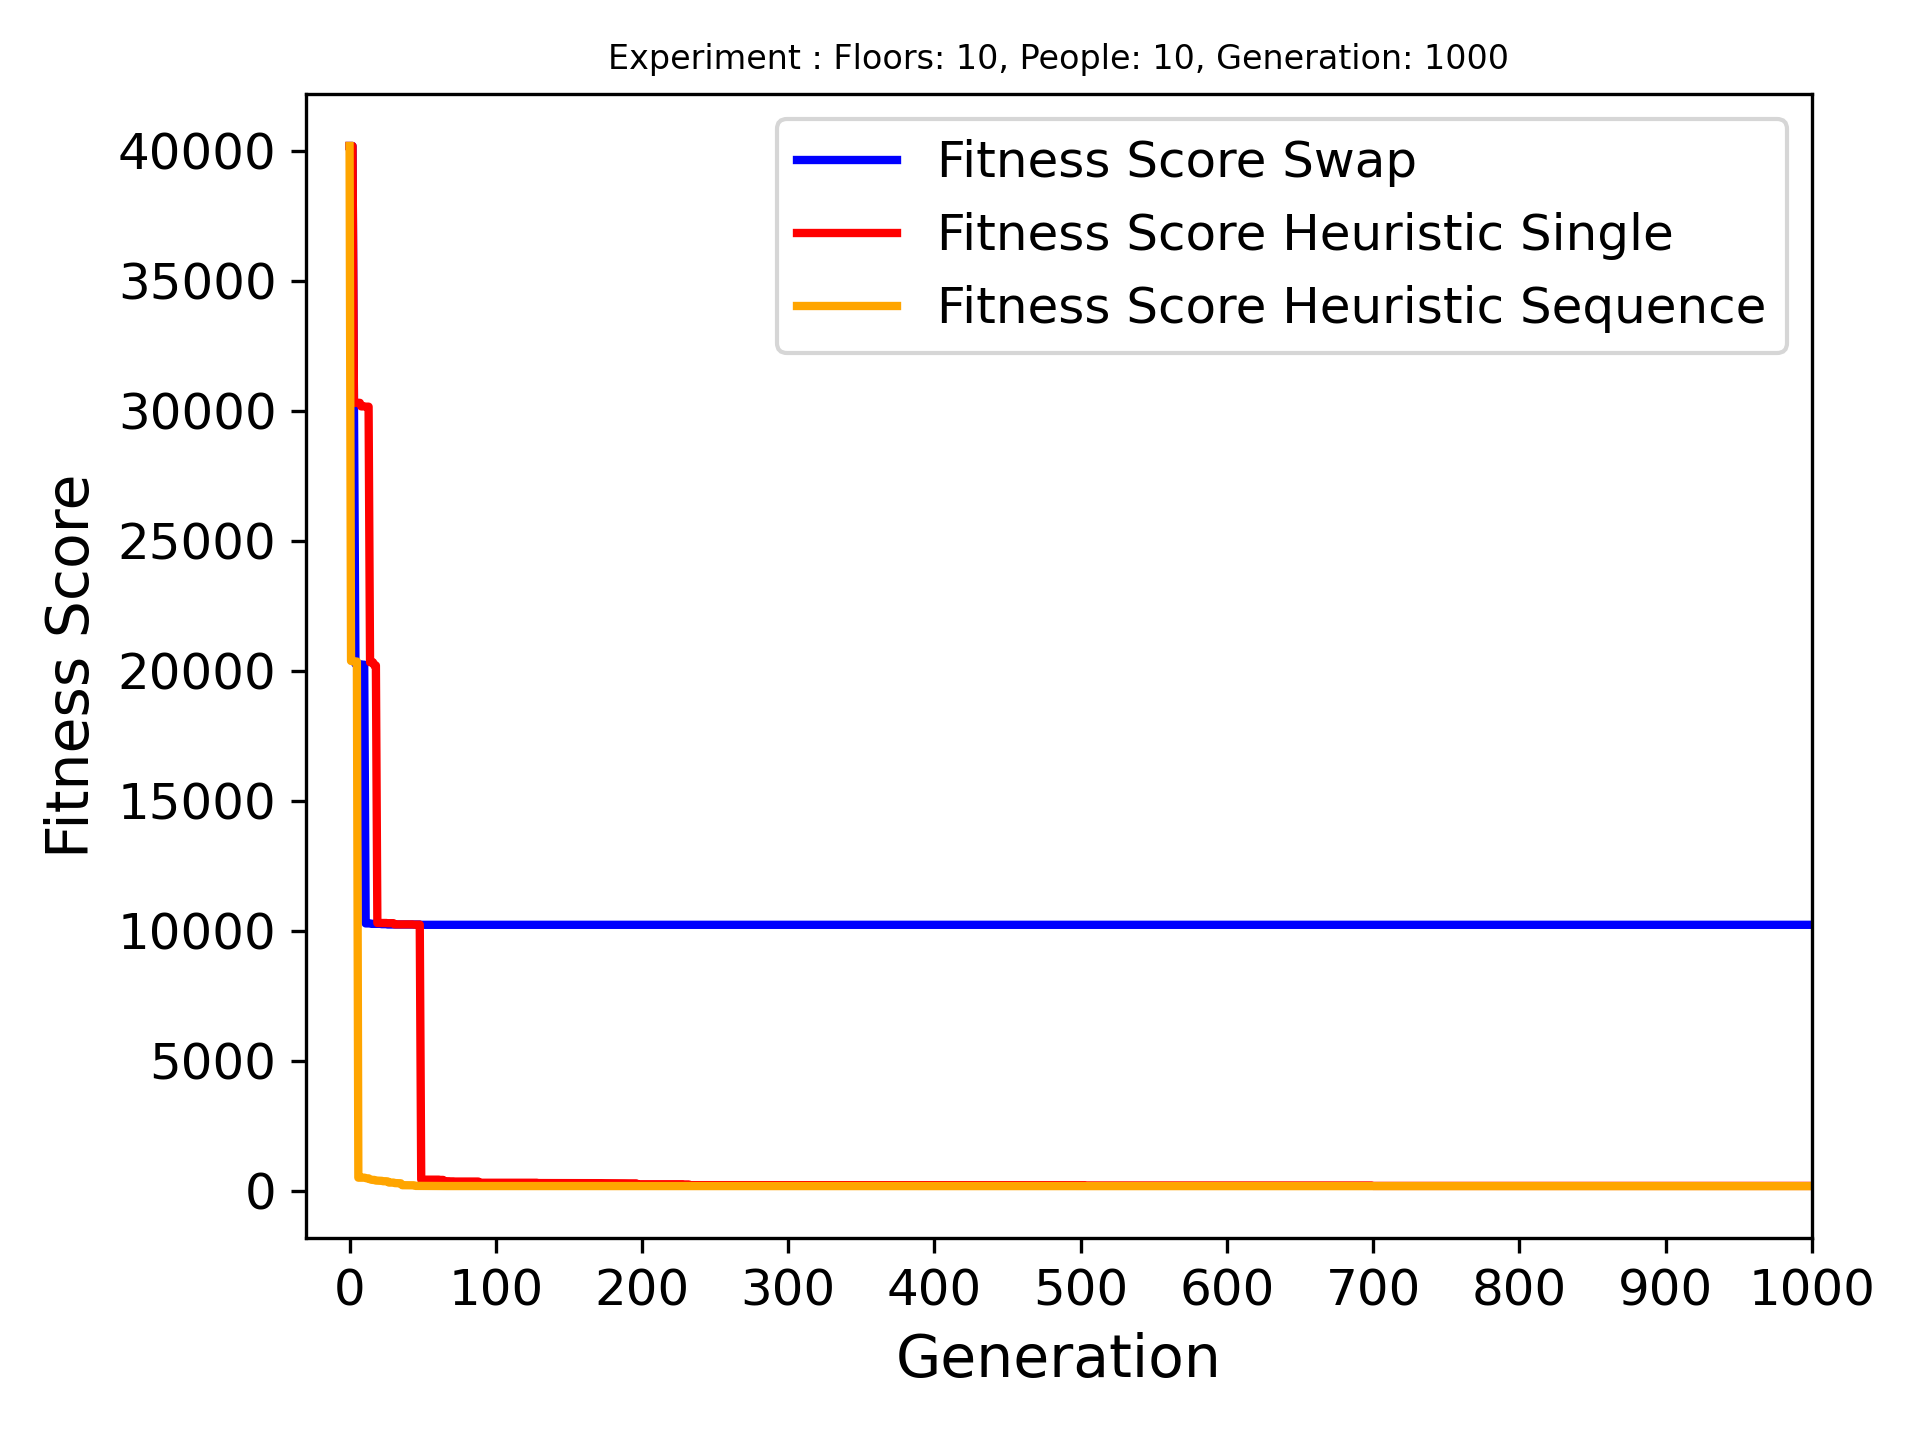
\includegraphics[width=\linewidth]{results/Building_Small/Mutation_0.1/Floors__10,_People__10,_Generation__1000_worst.png}
		\captionsetup{justification=centering,font=tiny}
		\caption{Score/Arrived/Length:\\\textcolor{blue}{10227/9/9}, \textcolor{red}{182/10/11}, \textcolor{orange}{172/10/11}.}
		\label{fig:Building Small worst}
	\end{subfigure}
	\hfill
	\begin{subfigure}[b]{0.49\linewidth}
		\centering
		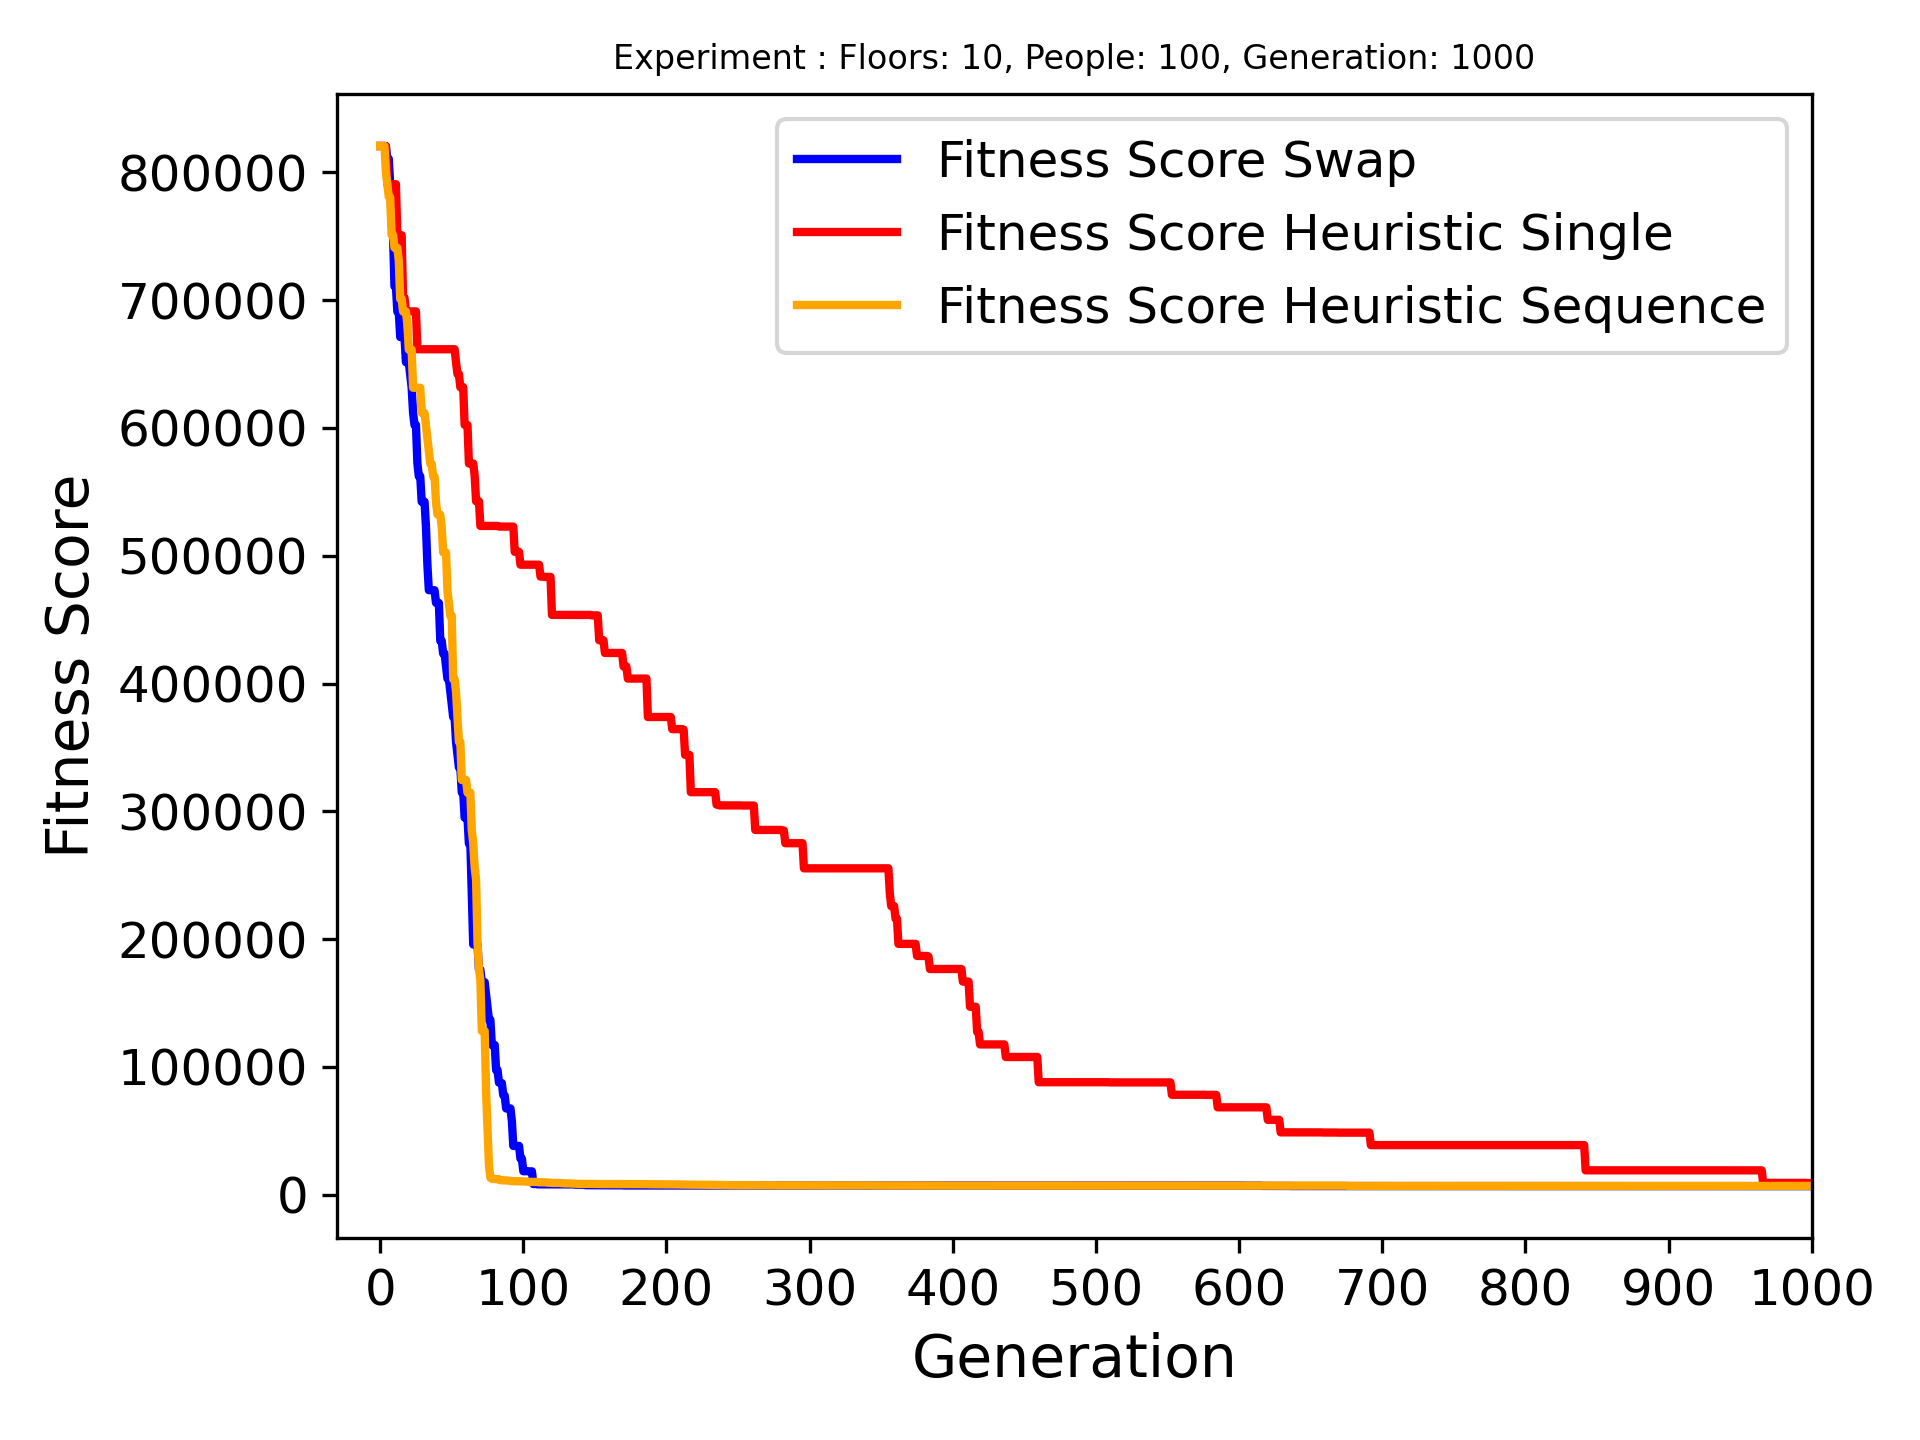
\includegraphics[width=\linewidth]{results/Building_Small/Mutation_0.1/Floors__10,_People__100,_Generation__1000.png}
		\captionsetup{justification=centering,font=tiny}
		\caption{Score/Arrived/Length:\\\textcolor{blue}{6727/100/45}, \textcolor{red}{9113/100/61}, \textcolor{orange}{6880/100/52}.}
		\label{fig:Building Small 100 people}
	\end{subfigure}
	\captionsetup{font=scriptsize}
	\caption{Comparing worst and best case.}
	\label{fig:Building Small results}
\end{figure}

\newpage

\subsection{Building Medium}
As previously noted, the red crossover tends to perform worse the more people in the building instances and Figure \ref{fig:Building Medium results} illustrates this once again. In Figure \ref{fig:Building Medium worst} the blue crossover outperformed the orange one, that got stuck in a local minimum for an extended period. The orange crossover was also slower than the blue one. Conversely, Figure \ref{fig:Building Medium best} then shows a scenario where the blue one performed similarly to how it performed in \ref{fig:Building Medium worst} and the orange one reached an extraordinary low score of 121157 without getting stuck in a local minimum. This demonstrates that the orange crossover have both strong worst case and great best case. This further underlines that the orange crossover is the most reliable crossover of the three.

\begin{figure}[ht]
	\centering
	\begin{subfigure}[b]{0.49\linewidth}
		\centering
		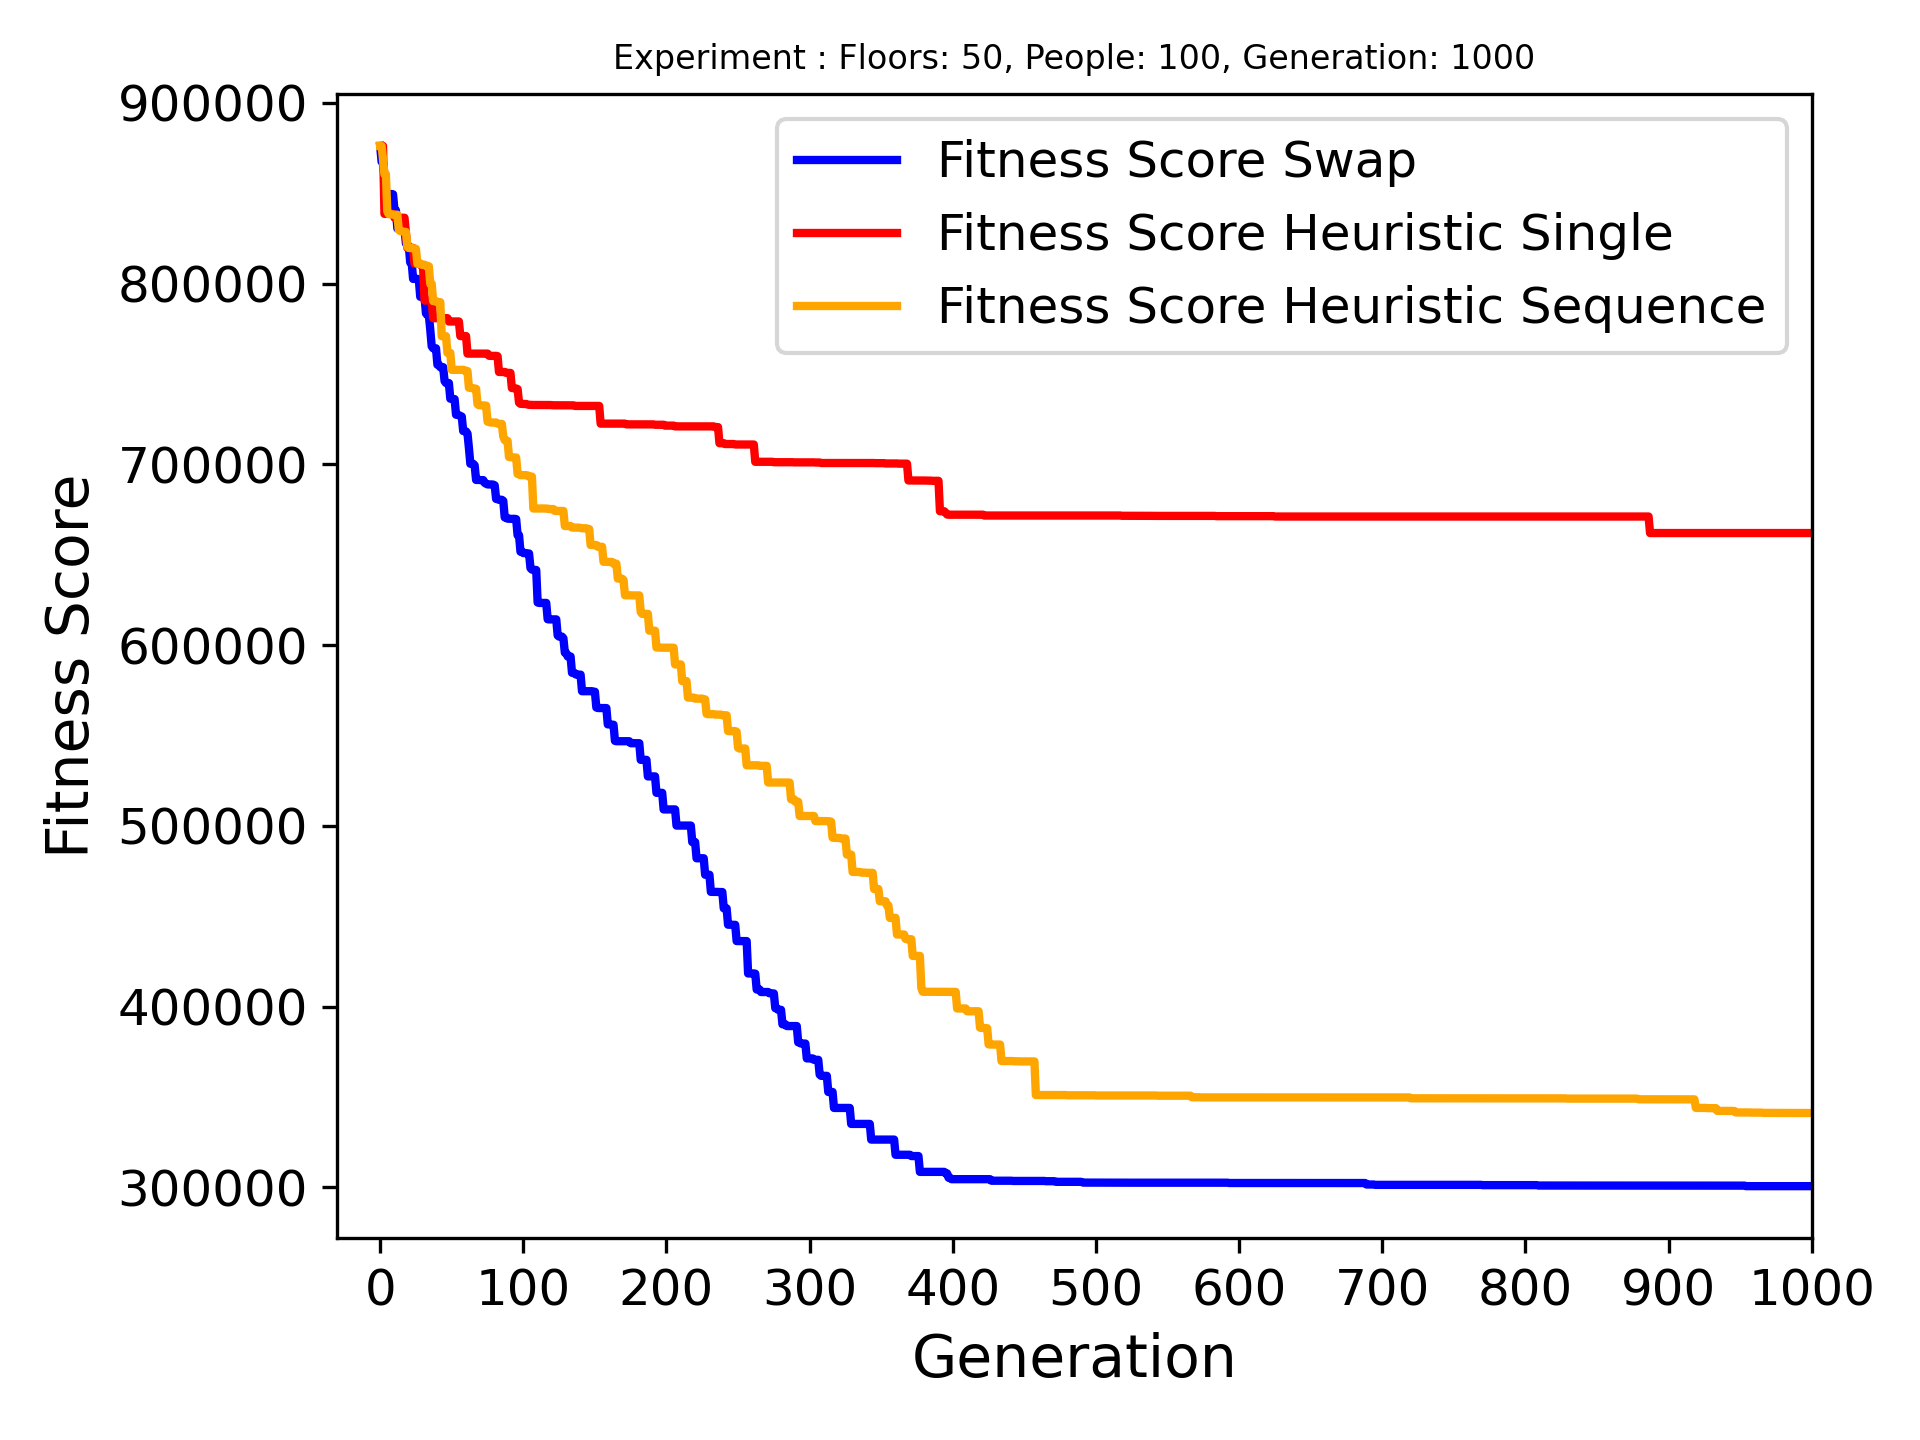
\includegraphics[width=\linewidth]{results/Building_Medium/Mutation_0.1/Floors__50,_People__100,_Generation__1000_4_worst.png}
		\captionsetup{justification=centering,font=tiny}
		\caption{Score/Arrived/Length:\\\textcolor{blue}{300697/74/69}, \textcolor{red}{661991/35/52}, \textcolor{orange}{341167/69/74}.}
		\label{fig:Building Medium worst}
	\end{subfigure}
	\hfill
	\begin{subfigure}[b]{0.49\linewidth}
		\centering
		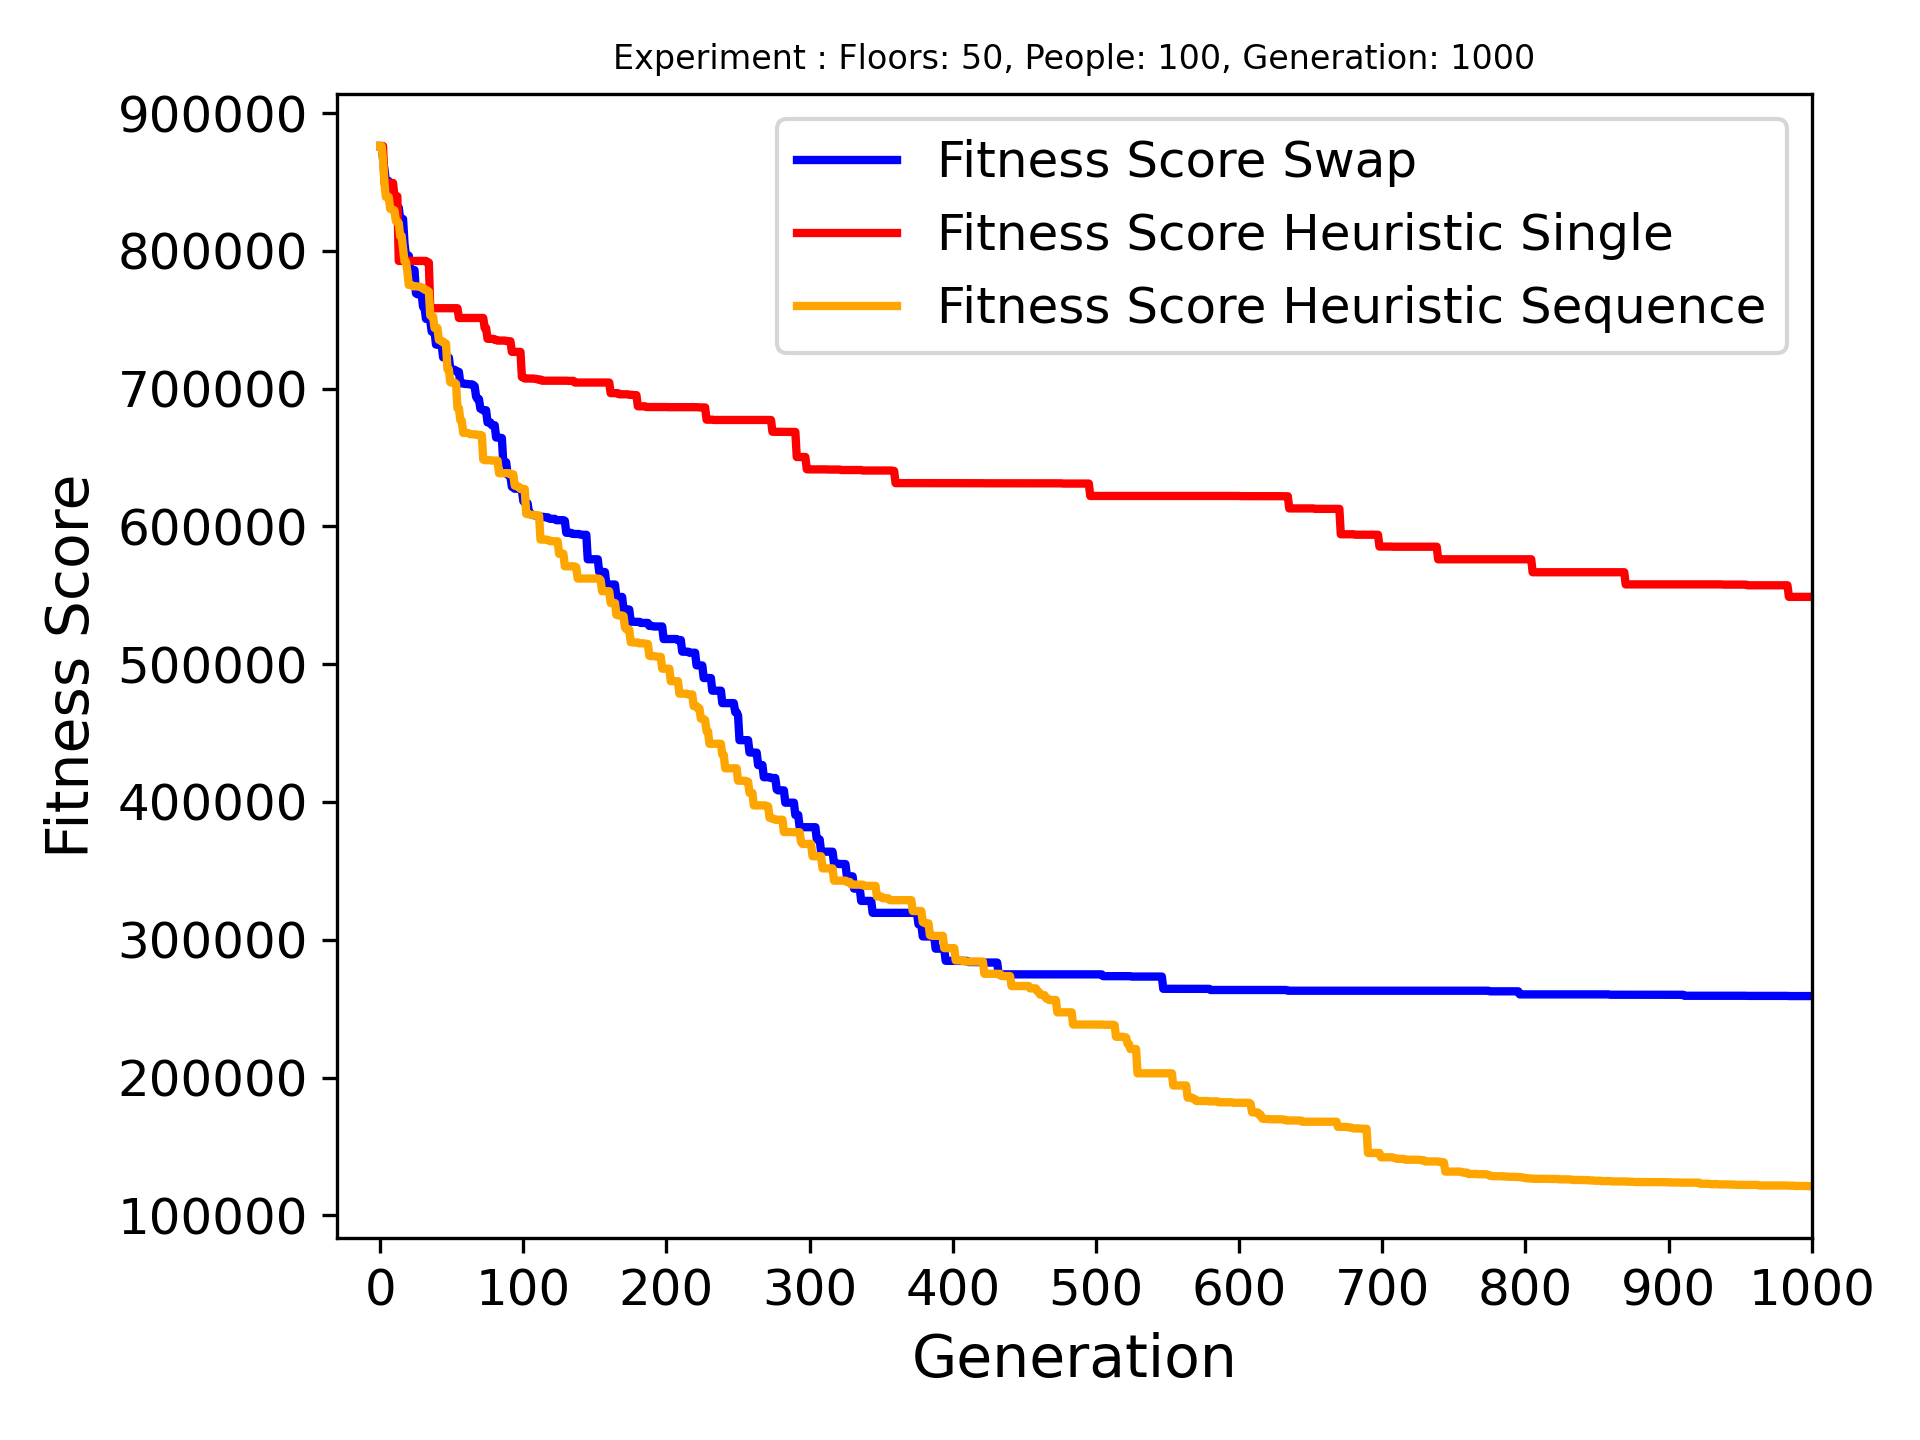
\includegraphics[width=\linewidth]{results/Building_Medium/Mutation_0.1/Floors__50,_People__100,_Generation__1000_1_best.png}
		\captionsetup{justification=centering,font=tiny}
		\caption{Score/Arrived/Length:\\\textcolor{blue}{259130/79/71}, \textcolor{red}{548857/48/59}, \textcolor{orange}{121157/94/124}.}
		\label{fig:Building Medium best}
	\end{subfigure}
	\captionsetup{font=scriptsize}
	\caption{Comparing worst and best case.}
	\label{fig:Building Medium results}
\end{figure}

\newpage

\subsection{Building Large}
After running all the buildings with a 10\% mutation rate, numerous experiments were executed with different rates. It was quickly determined that an increased mutation rate enabled the algorithm to find solutions that served all or almost all people much faster. Results in Figure \ref{fig:Building Large results} shows the best runs with mutation rates of 10\% and 60\%.

With a low mutation rate as in Figure \ref{fig:Building Large 0.1 best}, the best solutions achieved fitness scores around 500 000, whereas a higher rate tested in Figure \ref{fig:Building Large 0.6 best} yielded scores around 200 000. In the best run with a 10\% mutation rate, 66 people were served and the best run with a 60\% mutation rate served all 100 people. Not only that, it is clear that the algorithm reached acceptable solutions in a greater pace than before. Reason behind this is that to be able to serve as many people as possible the chromosomes have to mutate to become longer than number of floors. The higher mutation rate allowed the algorithm to reach this objective and escape local minimums faster. Further experimentation with mutation rates could potentially yield even better outcomes.

Similar results were obtained by increasing the number of generations and population size. The downside with this is that it requires more computational power and takes longer time to run. Therefore, a greater mutation rate was beneficial for fast feedback and limited hardware resources.

\begin{figure}[ht]
	\centering
	\begin{subfigure}[b]{0.49\linewidth}
		\centering
		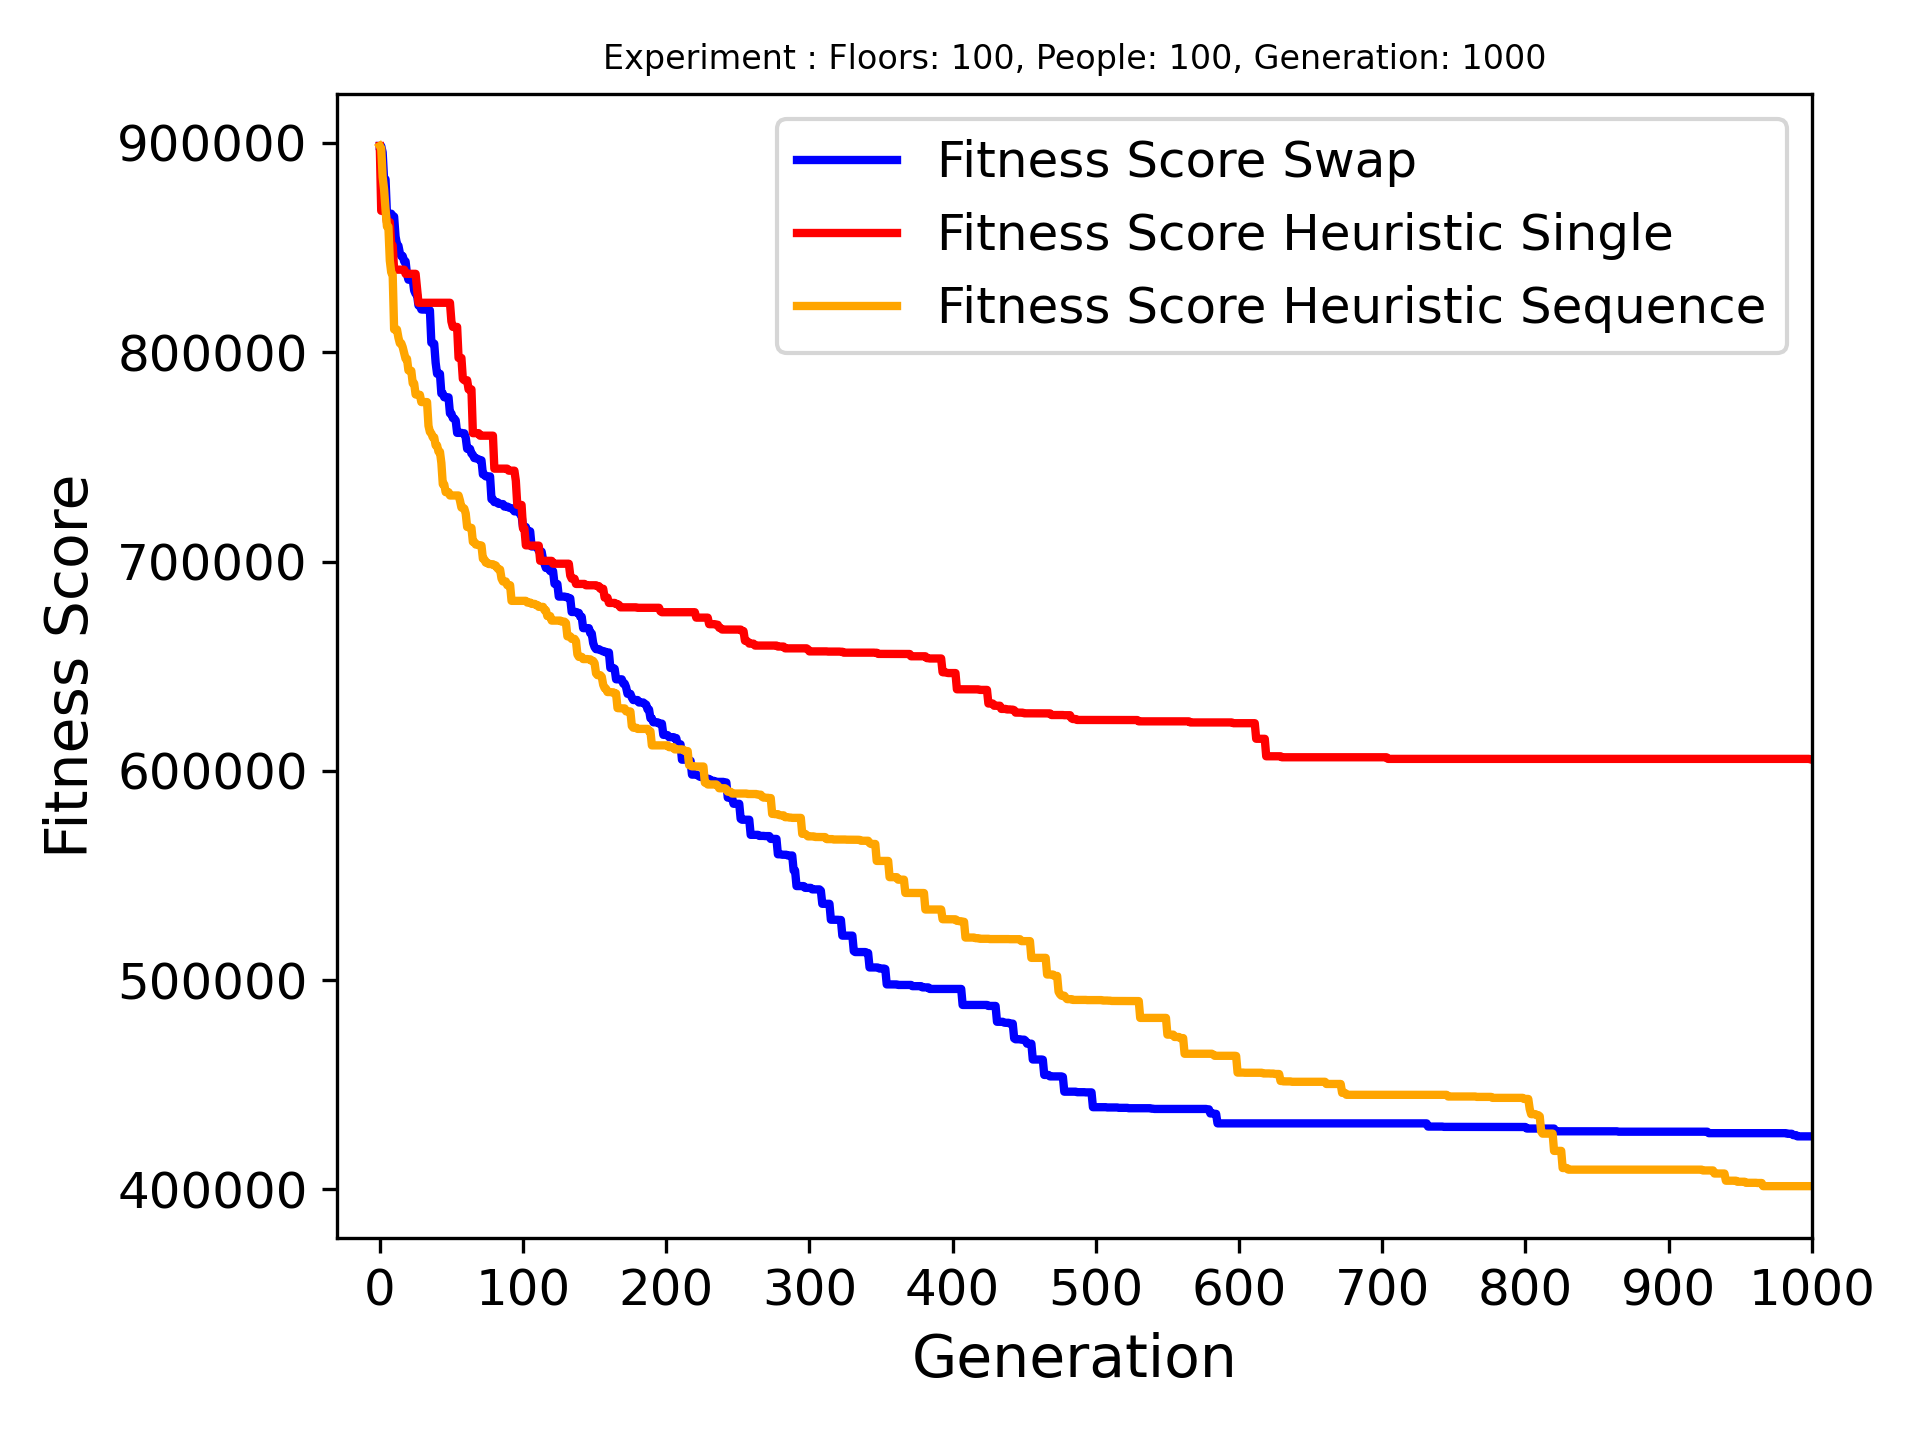
\includegraphics[width=\linewidth]{results/Building_Large/Mutation_0.1/Floors__100,_People__100,_Generation__1000_2_best.png}
		\captionsetup{justification=centering,font=tiny}
		\caption{Score/Arrived/Length:\\\textcolor{blue}{425352/67/80}, \textcolor{red}{605508/44/102}, \textcolor{orange}{401562/66/75}.}
		\label{fig:Building Large 0.1 best}
	\end{subfigure}
	\hfill
	\begin{subfigure}[b]{0.49\linewidth}
		\centering
		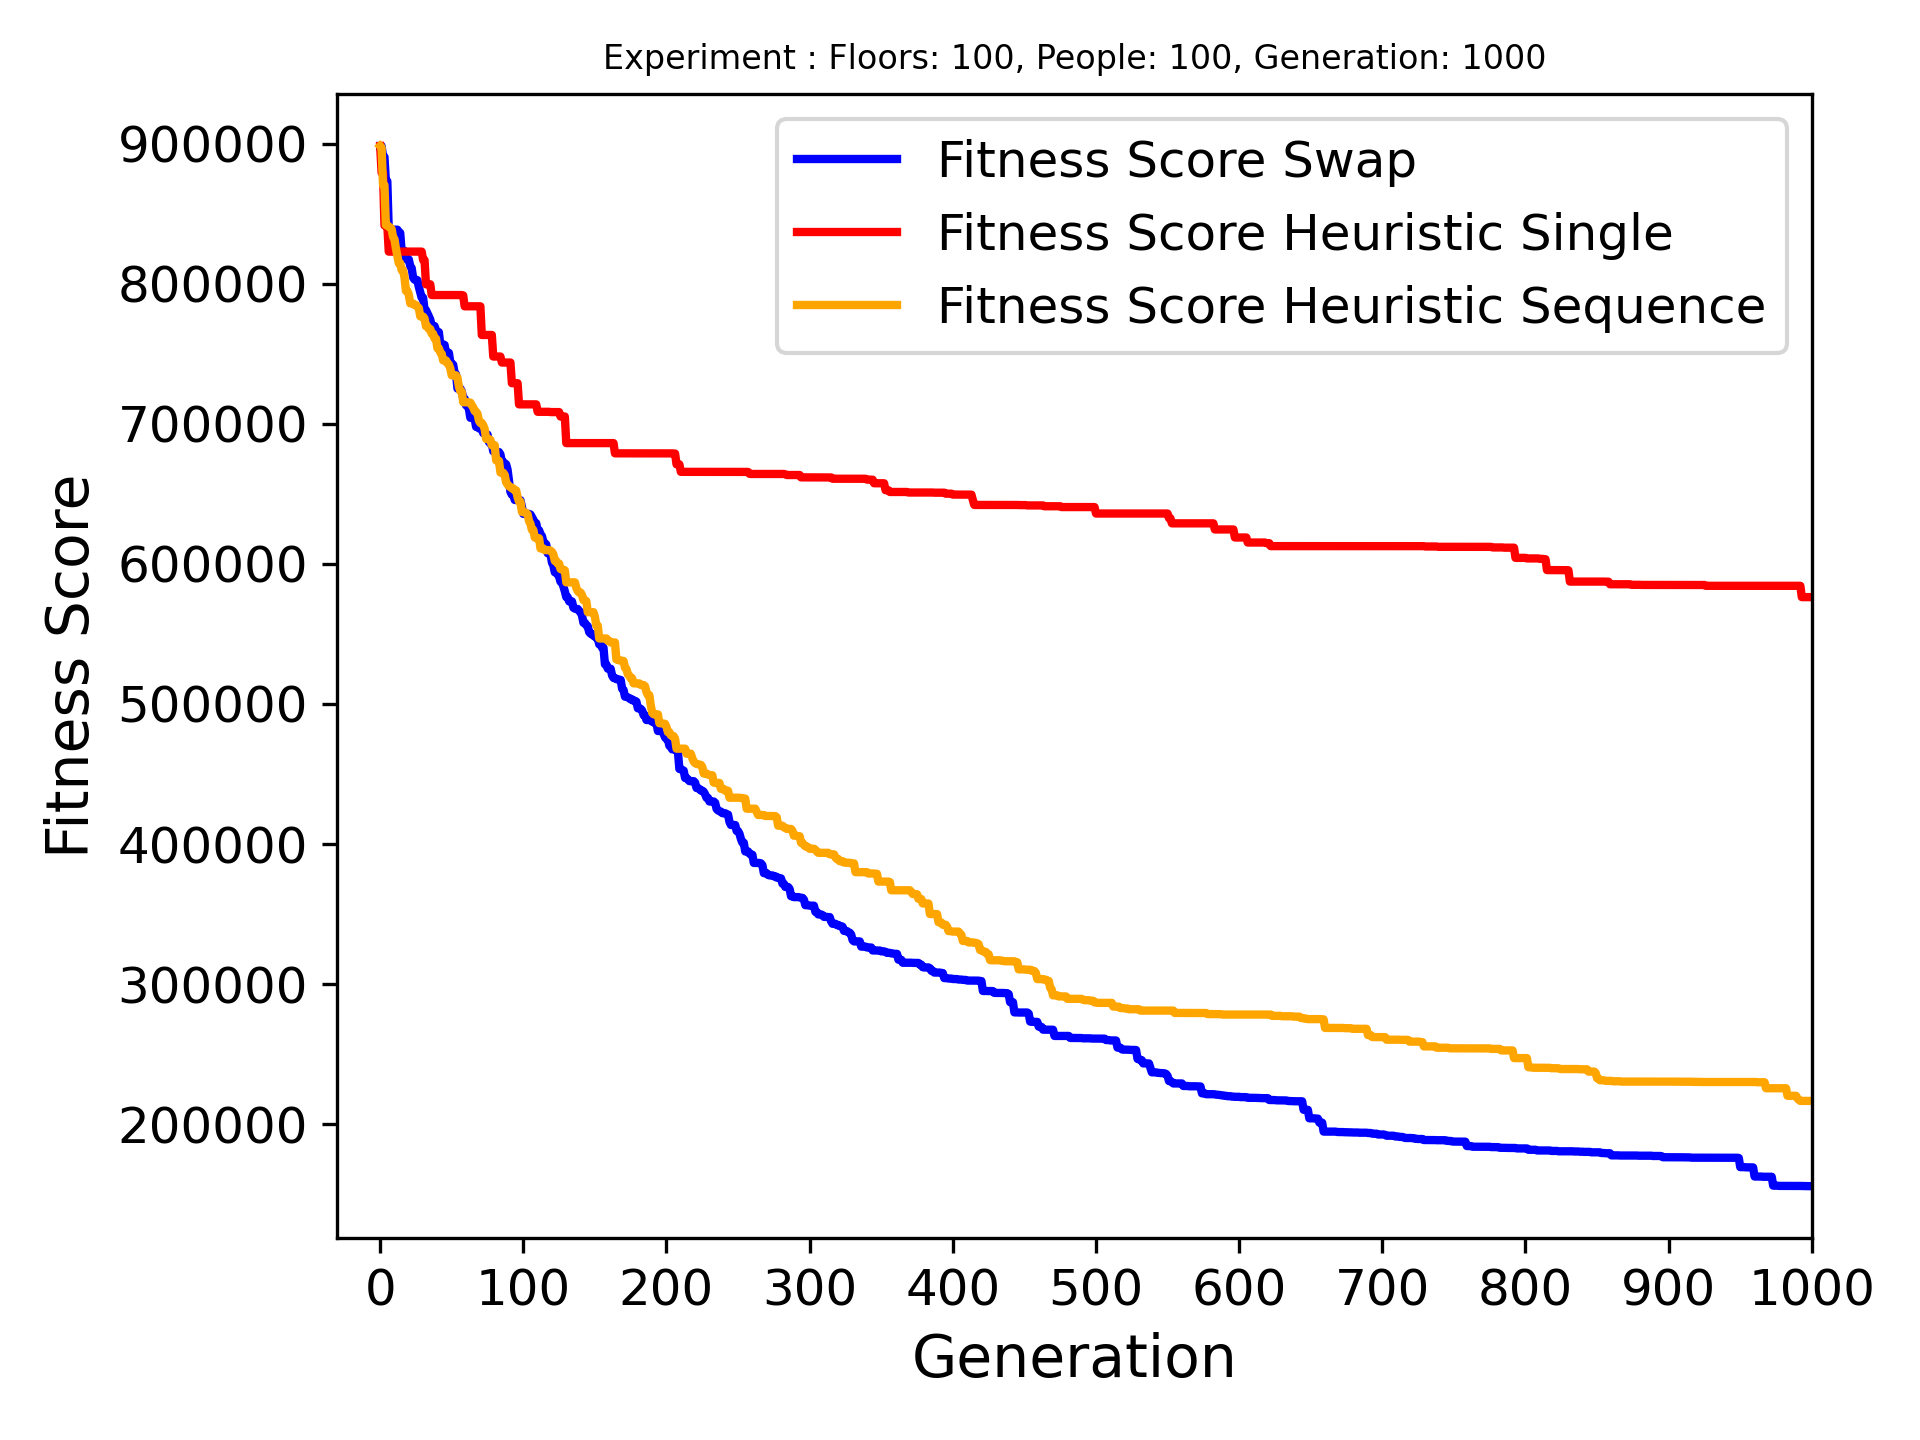
\includegraphics[width=\linewidth]{results/Building_Large/Mutation_0.6/Floors__100,_People__100,_Generation__1000_best.png}
		\captionsetup{justification=centering,font=tiny}
		\caption{Score/Arrived/Length:\\\textcolor{blue}{155619/100/151}, \textcolor{red}{576322/48/117}, \textcolor{orange}{216508/94/139}.}
		\label{fig:Building Large 0.6 best}
	\end{subfigure}
	\captionsetup{font=scriptsize}
	\caption{Comparing the best case for 10\% and 60\% mutation rate.}
	\label{fig:Building Large results}
\end{figure}

\newpage

\subsection{Building Special}
This special building used in experiments replicates the setup from a prior investigation on optimization techniques for the elevator dispatching problem \cite{ahmed2022investigation}. The people in this building has identical starting floors and destinations as the referenced study. Parameters for elevator population and number of generations are also aligned with values used for experimentation in the paper. This was done to ensure a fair comparison between the research. A minor difference is that the fitness function used in this study also gives an extra penalty for each extra floor a person travels in the elevator, as detailed in \ref{subsec:fitness_function}. Furthermore, the mutation used in this study also allows the chromosome length to increase and decrease.

The genetic algorithm in \cite{ahmed2022investigation} utilized Davis-order crossover, swap mutation, elitism, and a fitness function that measured the average time for all passengers to reach desired floor. The average result reported from running described algorithm, based on 5 runs was 279.1 seconds per traveler. In comparison, the average result in this study for 5 runs, was 305.1 seconds. Thus, this algorithm was approximately 26 seconds ($\approx$ 8.5\%) slower than the result in the paper. This difference could be explained by the extra penalty given in the fitness function. Additionally, it is possibly a coincidence, but one factor might have been that Davis-order crossover divides the chromosome into more segments while this crossover only splits it into two larger segments. Why this might affect the result is because when splitting the parent chromosome into two larger segments, parts of them will probably not contribute to a better result, and they will have a larger risk of remaining throughout more generations.


\newpage

\section{Conclusions}
\label{sec:conclusions}
% Author: Joel Scarinius Stävmo, Oskar Sundberg, Linus Savinainen, Samuel Wallander Leyonberg  and Gustav Pråmell
% Update: October 1, 2024
% Version: 1.0.0
% License: Apache 2.0

This paper mainly looked at different crossover functions impact on genetic algorithm ability to find solutions for various buildings configurations.

It started off with a fitness function that gave 10 points for each person served, which in the end promoted the algorithm to serve all people in the building.
The problem with this was that it tended to give long genomes because it was more beneficial to serve all people than to serve them quickly.
It was then changed to a fitness function that gave huge penalties for all people that weren't served by the elevator. It also increased the score by one for each additional unnecessary floor a person traveled in the elevator, worsening the overall result since a lower score is better.
This also made it possible to analyze the average waiting time and this was also the benchmark that most papers used for results in this kind of problems.

How different mutation functions would affect the results were not investigated in this paper. The implementation used 5 different ones that are randomly selected when a mutation occurred.
The mutation functions used were swapping a random element in a genome, increase the length of a genome, decrease the length of a genome and the combinations of swapping and increasing or decreasing the length of a genome.
These are all thoroughly explained in (3.1.3).

An approach that would have been interesting to test is to implement elements of heuristic operators into Davis-order crossover.
This would allow for more segments being made but also have the more dominant parent transfer more of its genes into the next generations.

Because the algorithm is not forced to find a solution where all people reach their destination floor, this implementation includes a time penalty discussed in (3.3), this is to incentivize the algorithm to serve all people to their destination floor.
Further research on the impact of this time penalty in relation to the number of people in the building and their configurations would be interesting.

A finding from this paper is that a higher mutation rate seems to be better. To determine this further research in this area is needed. Is a higher mutation rate better? If so, what is the optimal range?

In addition, this report does not focus on the selection algorithm for the problem. Further research on which selection algorithm will perform best for the problem at hand would be of interest.
Also, it could be interesting to investigate how other mutation functions could impact the results.

\newpage

\appendix
\section{Appendices}
\label{sec:appendices}
% Flowchart from paper
\begin{figure}[h]
    \centering
    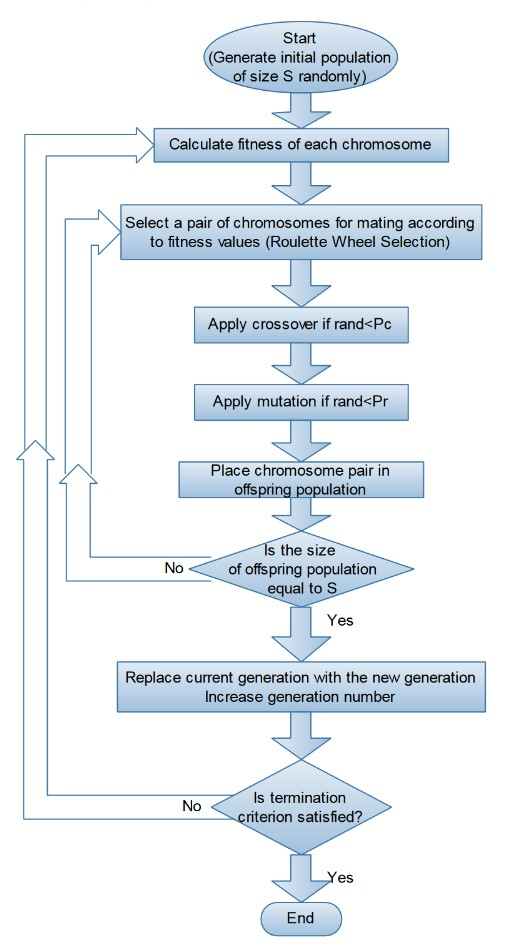
\includegraphics[width=0.5\textwidth]{figures/flowchart.jpg}
    \caption{Flowchart from \cite{tartan2016flow}}
    \label{fig:flowchart}
\end{figure}

\newpage

\bibliographystyle{ieeetr}
\bibliography{references}

\end{document}
